\chapter{How to Write a Novel: My Proven 12-Step Process}

This lecture contains no blackboard derivation, but it does contain something structurally close to one. Jenkins takes the beginner's diffuse fear about writing a novel and turns it into a sequence of constraints, tests, and update rules. The order matters. We begin by defining the object, then we choose the project, then we decide how it will be carried, how it will be seen, how it must begin, and how it must be driven to its point of maximum pressure before it resolves.

\begin{remark}
The displayed formulas in this chapter are cautious reconstructions of the lecture's procedural logic. They are not transcriptions of on-screen notation; they simply make the structure of the advice explicit.
\end{remark}

\section{From Fear to Method}

Jenkins opens by clearing the ground. Before process, before craft, before motivation, he tells us what object is under discussion. In the present lecture, a novel is fiction. That sounds elementary, but it is the right first move, because it fixes the target and prevents the talk from dissolving into a looser discussion of writing in general.

\begin{definition}
In the sense of this lecture, a novel is a work of fiction.
\end{definition}

\begin{equation}
\text{novel}=\text{fiction}.
\end{equation}

From there the lecture pivots at once to the real obstacle. The listener has an idea, wants to write, and may even have been told that he or she has a gift for words; but privately there is fear that an entire novel is too large to finish, or too difficult to finish well. Jenkins does not answer that fear with a vague appeal to inspiration. He answers it by promising a repeatable process.

He also inserts two motivational beats that are important to preserve. First, even a practiced novelist continues to worry about whether an idea can carry a book and whether the writing will be good enough. Second, he asks the listener to stay with the lecture to the end, because there will be a bonus step on revision and a checklist for checking every word before submission. So already the lecture is doing what it recommends: it establishes the problem, promises a structure, and sets up a payoff.

\subsection{Question \& Answer}

\paragraph{Question.} How do we proceed if we fear that we do not have what it takes to write a whole novel?

\paragraph{Answer.} We do not wait for fear to vanish. We replace an indefinite ambition with a concrete sequence of steps. Jenkins's first promise is not that writing will become easy, but that it can become intelligible and repeatable.

\section{Choosing the Story and Surviving the Middle}

The first substantive question is selection. We may have many story ideas; Jenkins treats that not as the solution but as the initial condition. The problem is to choose the one idea that has enough weight to carry a book and enough emotional force to keep us at work when the excitement of the first pages has worn off.

He gives a practical scale at once: a winning idea must be able to carry a novel of substantial length, not just a clever opening, a scene, or a premise. Structurally, the novel is first partitioned into three regions:

\begin{equation}
\text{Opener} \to \text{Middle} \to \text{Ending}.
\end{equation}

The lecture's most memorable phrase in this early section is the one that names the difficult region.

\begin{definition}
The marathon of the middle is the long central stretch of the novel between opener and ending, where drama, tension, conflict, action, and setups demanding payoffs must be sustained.
\end{definition}

This is where Jenkins becomes more exact than the usual advice to ``write what you love.'' It is not enough that an idea spark at the beginning. It must be able to survive duration. An idea is tested not by its novelty alone, but by whether it continues to draw us back after the opening energy fades and before the ending is in sight.

The lecture then gives a remarkably useful response test. Jenkins treats the writer's own reaction as a local detector for the story's energy on the page:

\begin{align}
\text{if it bores us} &\Rightarrow \text{it puts the reader to sleep},\\
\text{if it feels flat} &\Rightarrow \text{we lose the reader},\\
\text{if it chokes us up} &\Rightarrow \text{the reader sobs},\\
\text{if it makes us smile} &\Rightarrow \text{the reader is warmed}.
\end{align}

This is not mere sentiment. It is an operational rule. Jenkins is saying that the writer's own felt response is evidence about whether the narrative is still carrying force.

\subsection{Question \& Answer}

\paragraph{Question.} How do we know which story idea can actually carry a novel?

\paragraph{Answer.} We test the idea against endurance. The winning idea is the one for which our passion survives the middle, the one that still pulls us to the keyboard when the work becomes repetitive, difficult, or discouraging.

\paragraph{A worked filter.} The lecture's selection rule can be stated as a short update procedure:

\begin{enumerate}
\item Start with a set of candidate ideas.
\item Ask which one continues to draw us back to the work.
\item Test that idea against the middle, not merely against a strong opening image.
\item Keep the idea whose passion remains durable under frustration and repetition.
\end{enumerate}

\section{Temperament, Structure, and the Classical Sequence}

Once the project is chosen, the lecture asks how we are to work on it. Jenkins introduces the familiar distinction between outliner and pantser. The outliner wants the architecture laid out in advance; the pantser begins from a seed and discovers the path by writing. He invokes Stephen King as the best-known example of the second temperament.

But the lecture does not let this become a tribal argument. Jenkins explicitly dissolves the false opposition: neither method is intrinsically better. Many writers are hybrids, wanting both the security of some map and the freedom of discovery. He himself identifies strongly with the pantser side, yet he immediately adds that he never starts without some idea of what he is doing. That qualification is crucial, because it carries us into the talk's first real formal model.

\subsection{Question \& Answer}

\paragraph{Question.} Must we outline, or can we discover the story as we go?

\paragraph{Answer.} We may discover a great deal as we go, but discovery does not abolish structure. Whatever our temperament, the novel still needs a carrying sequence robust enough to prevent the work from stalling after the opening pages.

Jenkins then cites Dean Koontz's ``classic story structure.'' This is the lecture's clearest algorithmic backbone, and we should preserve it in a compact symbolic form:

\begin{equation}
T_0 \to T_1 \to T_2 \to T_3,
\end{equation}
with
\begin{align}
T_0&=\text{terrible trouble introduced early},\\
T_1&=\text{progressively worsening trouble},\\
T_2&=\text{the predicament appears hopeless},\\
T_3&=
\begin{aligned}[t]
\text{the hero wins through developed} \\
\text{strength and insight}
\end{aligned}.
\end{align}

\begin{figure}
\centering
\resizebox{\linewidth}{!}{%
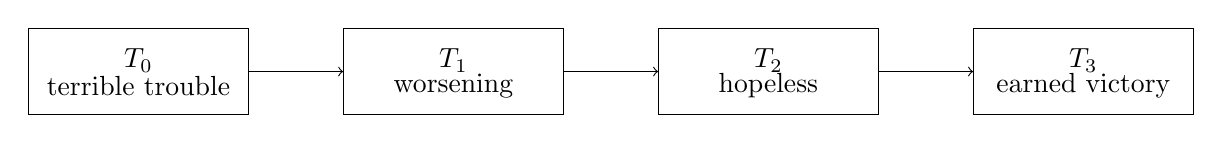
\begin{tikzpicture}
\draw (-1.4,0.55) rectangle (1.4,-0.55);
\node at (0,0.14) {$T_0$};
\node at (0,-0.18) {terrible trouble};

\draw (2.6,0.55) rectangle (5.4,-0.55);
\node at (4.0,0.14) {$T_1$};
\node at (4.0,-0.18) {worsening};

\draw (6.6,0.55) rectangle (9.4,-0.55);
\node at (8.0,0.14) {$T_2$};
\node at (8.0,-0.18) {hopeless};

\draw (10.6,0.55) rectangle (13.4,-0.55);
\node at (12.0,0.14) {$T_3$};
\node at (12.0,-0.18) {earned victory};

\draw[->] (1.4,0) -- (2.6,0);
\draw[->] (5.4,0) -- (6.6,0);
\draw[->] (9.4,0) -- (10.6,0);
\end{tikzpicture}
\par}%
\end{figure}

This schematic figure is not visual evidence from the video; it is a cleaned reconstruction of the sequence Jenkins states in words. It tells us what the lecture needs it to tell us: narrative pressure is not random. It is built by introducing trouble early, worsening it step by step, refusing premature relief, and resolving it only through a transformed protagonist.

Jenkins closes this structural passage with a strong imperative that prepares the next steps: whatever basic form we use, we must grab readers by the throat from the beginning and never let go. Only then does he move to character.

\section{Character, Research, and Point of View}

The lecture now passes from engine to carrier. A plot structure by itself is empty unless there are characters who can bear its pressure. Jenkins's first demand is that the protagonist have an arc. By the end, the lead must be a different, preferably better, person. The later victory therefore cannot be an arbitrary success; it must arise from development.

A second condition immediately follows. The protagonist should have flaws, but not such repulsive flaws that the reader is pushed away from the outset. On the opposing side, the antagonist must be formidable and compelling. Jenkins is very clear about the beginner's mistake here: the villain is not to be evil merely because the slot in the story requires a villain. Most villains think they are right. So the antagonist, too, needs intelligible motives.

The same principle extends outward. The important orbital characters must be more than stock figures from central casting. Jenkins mentions a longer question list for developing them, but the transcript becomes corrupted at exactly that point. We should therefore preserve only what remains stable: names should be distinct, initials should not blur together, and characters should look and sound different enough that the reader does not confuse them.

At this point the lecture introduces a useful pair of coupled variables. The lead character faces an outward problem, but comes alive through inward turmoil. The external goal and internal weakness must not be separated; the story works by driving them together.

Research enters next, and here the lecture is concrete. Fiction is invented, but it must still be believable. Even fantasy and science fiction must hold together internally if the reader is to suspend disbelief. Jenkins gives a compact ratio worth keeping:

\begin{equation}
\text{Research}=\text{flavor},\qquad \text{Story}=\text{main course}.
\end{equation}

He then names the kinds of resources a working novelist might actually use:

\begin{itemize}
\item atlases and world almanacs,
\item encyclopedias and search engines,
\item interviews, in person or by call,
\item even such ordinary tools as YouTube and thesauri.
\end{itemize}

The point is not glamour. The point is to get the geographical, cultural, and technological details right enough that the reader does not fall out of the story. Jenkins also adds the important caveat that with futuristic fiction we will invent many technical details, but even invented systems must make sense and remain consistent.

From research the lecture moves naturally to point of view. This, Jenkins insists, is not just a grammatical choice among first, second, and third person. It is the decision about who functions as the story's camera. Let \(s\) denote a scene and \(\mathrm{POV}(s)\) its perspective character. Then the lecture's operative restriction can be stated as

\begin{equation}
|\mathrm{POV}(s)|=1.
\end{equation}

Jenkins states the rule in prose: one perspective character per scene, while adding that he personally prefers one per chapter and ideally one per novel. Once that bound is set, the channel of narrative information is bounded as well:

\begin{equation}
\mathrm{Info}(s)=
\left\{
\begin{aligned}
&\text{see, hear, touch,} \\
&\text{smell, taste, think}
\end{aligned}
\right\}_{\mathrm{POV}(s)}.
\end{equation}

Again, that notation is ours, not his, but it faithfully summarizes the lecture: the narration may convey what the viewpoint character perceives and thinks. We are in that mind, using that character's senses and emotions. Jenkins then resolves a common beginner's misunderstanding. This restriction does \emph{not} force us into first person. Third person limited remains fully compatible with a single perspective channel, and in fact it is the modern default. What he warns against is casual omniscience, the old habit of hopping in and out of multiple heads inside a single scene.

\subsection{Question \& Answer}

\paragraph{Question.} How does point of view constrain what the novel can reveal?

\paragraph{Answer.} Point of view is an information boundary, not an impoverishment. Once we choose the scene's perspective character, the prose is limited to what that character can perceive, infer, remember, and think. That still allows us to reveal orbital characters, but only through the pressure of a single consciousness at a time.

\section{Beginning in the Midst of Things and Triggering the Reader's Mind}

Just before step six, Jenkins briefly reminds the listener of the promised bonus step at the end. That reminder is not accidental; it keeps the procedural frame alive even while the lecture turns to style. Then he begins the next movement with a classical term: \emph{in medias res}, in the midst of things.

He is careful to head off a predictable confusion. Beginning in the midst of things does not necessarily mean gunfire or a chase. It means that we do not begin with inert explanation, scene-setting, or background when the story ought already to be moving. The opening must carry forward pressure. Jenkins states the rule with characteristic bluntness: the goal of every sentence, indeed of every word, is to force the reader to read the next.

We may write that local law of motion as

\begin{equation}
\text{sentence } n \Rightarrow \text{desire to read sentence } n+1.
\end{equation}

He then classifies four kinds of opening line: the surprise opener, the dramatic statement, the philosophical opener, and the poetic opener. The quoted examples in the lecture are used not as literary ornaments but as demonstrations of different kinds of forward pull. A clock striking \(13\) violates expectation. A sudden act of violence opens a dramatic gap. A philosophical generalization invites us to test it. A strange poetic image destabilizes tone and makes us curious about the world that contains it.

But Jenkins does not let the lecture stop at first lines. A strong opener is necessary and not sufficient. Many novels begin with energy and then immediately sink back into explanation. So he pushes on to the next beat: the theater of the reader's mind.

The claim here is one of the strongest in the lecture. As writers, we are not trying to force readers to see the scene exactly as we see it. We are trying to trigger their own imaginative construction. We suggest enough, and then the reader's mind does the rest. This is where the lecture turns to the famous distinction between telling and showing:

\begin{equation}
\begin{aligned}
\text{Telling} &\Rightarrow \text{reader is informed},\\
\text{Showing} &\Rightarrow \text{reader deduces}.
\end{aligned}
\end{equation}

\subsection{Question \& Answer}

\paragraph{Question.} What does it really mean to show rather than tell?

\paragraph{Answer.} It means that we replace an abstract report with concrete evidence from which the reader can infer the hidden state. The reader is not merely receiving a fact; the reader is helping to build the scene.

\paragraph{A worked update rule.} Jenkins's conversion procedure may be written as follows:

\begin{enumerate}
\item Identify the abstract report: tall, angry, cold, frightened, and so on.
\item Ask what another character, or the reader, could actually observe.
\item Replace the abstract predicate with those observable cues.
\item Remove the direct report once the evidence is carrying the meaning by itself.
\end{enumerate}

His two clearest examples survive well in note form:

\begin{align}
\text{``He was tall''} &\to
\begin{aligned}[t]
\text{others look up at him;} \\
\text{he ducks through a doorway}
\end{aligned},\\
\text{``He was angry''} &\to
\begin{aligned}[t]
\text{his face flushes, his throat tightens,} \\
\text{his voice rises, his fist hits the table}
\end{aligned}.
\end{align}

The reader completes the last step internally. That is why showing is not just prettier prose. It is a way of giving the reader a role in the experience.

\section{Escalation, the Bleakest Moment, and the Final Discipline}

By the time Jenkins reaches step eight, the earlier structure is ready to return in concrete form. The hero has been launched into trouble; now the rule is that every attempt to get out should make matters worse. Here the lecture gives its strongest maxim:

\begin{equation}
\text{Conflict}=\text{engine of fiction}.
\end{equation}

Jenkins drives the point home by offering a deliberately over-comfortable counterexample: a private investigator with looks, health, money, equipment, a happy home, a fine office, and a rich client carrying a juicy case. Unless the novel is parody, such ease kills narrative force. His corrective is brutally simple: remove supports. Take away ease, money, security, equipment, health, domestic stability. Once the protagonist is under genuine pressure, the story comes alive.

We can restate the escalation rule as a short derivation:

\begin{enumerate}
\item Begin with real trouble.
\item Let each attempted solution intensify the situation.
\item Strip away supports rather than adding conveniences.
\item Use rising pressure to keep the reader at the edge of the page.
\end{enumerate}

From there the lecture advances to step nine, the bleakest moment. Jenkins borrows Angela Hunt's phrase for the point at which even the writer wonders how the story can be written out of its own trap. The lecture's own example is melodramatic on purpose: the reformed lover, now devoted and apparently changed, destroys everything the night before the wedding. That is the point of the example. The situation must look irreparable.

\begin{definition}
The bleakest moment is the local nadir of the plot, the point at which the protagonist's predicament appears hopeless even to the writer.
\end{definition}

This gives the lecture's late chain:

\begin{equation}
\begin{aligned}
\text{trouble}
&\to \text{worsening trouble} \\
&\to \text{bleakest moment} \\
&\to \text{climax} \to \text{ending}.
\end{aligned}
\end{equation}

\subsection{Question \& Answer}

\paragraph{Question.} How hopeless should the hero's situation become before the ending can feel earned?

\paragraph{Answer.} Hopeless enough that no easy path out remains visible. Jenkins is emphatic here: do not invent a soft escape, do not inject a miracle, do not give the protagonist a break merely because the pressure has become uncomfortable. The whole function of the bleakest moment is to force action through whatever new muscle and insight the story has built.

That answer prepares the distinction on which the lecture then insists:

\begin{equation}
\text{Climax} \neq \text{Ending}.
\end{equation}

The climax is the final test, the peak of confrontation, the point at which the book-length setups are paid off. The ending comes after it. It is quieter, but not dispensable. Jenkins gives two criteria for a successful ending: it puts the reader first, honoring the reader's investment, and it keeps the hero on stage through the last word. In other words, the novel cannot simply stop once the fireworks are over; it must still land.

The lecture then closes by returning from fictional process to writerly process. The bonus step is not an appendix. It completes the logic of the whole talk. Just as the novel needs ordered stages, so does the work of writing it. Jenkins's final rule is

\begin{equation}
\text{Drafting} \neq \text{Editing}.
\end{equation}

The first draft is to be written with the inner critic muted. Cliches, rough transitions, and logical infelicities are not to be solved on the spot if solving them destroys motion. Revision comes later, in a separate mental mode. The lecture's final update rule is therefore this:

\begin{enumerate}
\item Draft without stopping for perfection.
\item Allow roughness to remain during the drafting pass.
\item Return in a separate revision pass.
\item Fine-tune word by word only after the drafting motion is complete.
\end{enumerate}

The promised twenty-one-part checklist belongs to that second mode. Since the transcript does not preserve its contents, we preserve only its role: it is a revision instrument, not a drafting instrument.

\section{Summary}

The lecture begins with fear and ends with discipline. Along the way it turns a large, blurred ambition into a structured progression: define the object, choose the one durable idea, distinguish temperament from structure, give the story a carrying sequence, build characters who can bear pressure, make the world believable, restrict the prose to a coherent point of view, begin in motion, let the reader infer rather than merely receive, increase conflict, drive the story to its bleakest moment, separate climax from ending, and separate drafting from editing.

So the chapter's deepest lesson is not that writing can be reduced to a formula, but that it can be stabilized by one. We choose the project that can survive the middle, we constrain the narrative so the reader can truly enter it, and we let the conflict deepen until the ending is not merely arrived at, but earned.
